\documentclass{article} % \documentclass{} is the first command in any LaTeX code.  It is used to define what kind of document you are creating such as an article or a book, and begins the document preamble

\usepackage{amsmath} % \usepackage is a command that allows you to add functionality to your LaTeX code
\usepackage{graphicx}
\graphicspath{ {./images/} }
\title{DSP Chapter 1 Notes} % Sets article title
\author{Hunter Mills} % Sets authors name
\date{\today} % Sets date for date compiled

% The preamble ends with the command \begin{document}
\begin{document} % All begin commands must be paired with an end command somewhere
    \maketitle % creates title using information in preamble (title, author, date)
    
    \section{Classification of Signals} % creates a section
    
    \subsection{Multichannel and Multidimensional Signals}
    
    A signal is described by a function of one or more independent variables. The value of the function can be real, complex, or a vector. For example,
    a earthquake creates primary, secondary and surface waves. These can be described by a \textbf{multichannel signal}, $S_3(t)$.
    \begin{equation}  
	S_3(t) = \begin{bmatrix}
			s_{1}(t) \\
			s_{2}(t) \\
			s_{3}(t)
			\end{bmatrix}  
    \end{equation}
    
    If the signal is a function of a single independent variable, it is a \textbf{one-dimensional signal}, whereas a signal is a \textbf{M-dimensional signal} if
    it is a function of M independent variables. A TV would be a 3-Dimensional and 3 Channel signal with $I_r(x,y,z), I_g(x,y,z)$ and $I_b(x,y,z)$.
    \begin{equation}  
	I(x, y, t) = \begin{bmatrix}
			i_{r}(x,y,x) \\
			i_{b}(x,y,x) \\
			i_{g}(x,y,x) \\
			\end{bmatrix} 
    \end{equation}
    
    \section{Frequency in CT and DT signals}
    \subsection{CT Sinusoidal Signals}
    An example of a time domain sinusoidal signal is
    \begin{equation}  
	x_a(t) = A\cos(\Omega t + \theta), \;\;\;-\infty < t < \infty     
    \end{equation}
    The subscript a denotes an analog signal. This function is defined by amplitude (A), frequency($\Omega$ in rad/sec, or Hz) and phase ($\theta$). Instead of using $\Omega$, F is also used
    as frequency meaning cycles per second or hertz.
    \begin{equation}  
	\Omega = 2 \pi F    
    \end{equation}
    
    \begin{figure}[h]
    \centering
	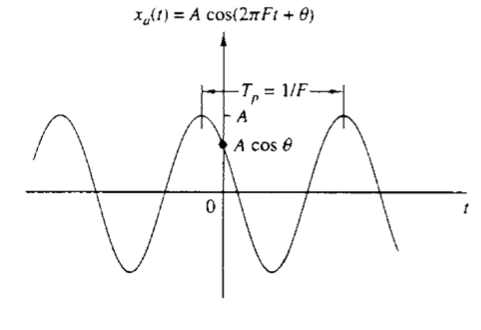
\includegraphics[width=10cm]{ct_sin}
	\caption{Example of analog sine wave}
	\end{figure}
	An analog sinusoidal signal is characterized by the following properties:\\
	\textbf{A1.} For every fixed value of the frequency F, the sine wave will be periodic.
	\begin{equation}  
	x_a(t + T_p) = x_a(t)  
    \end{equation}
    where $T_p = 1/F$ is the fundamental period of the sine wave. If a function of multiple sine waves added together, one must find the lowest common multiple of the frequencies. If there is none, the function is not periodic.\\
    \textbf{A2.} CT sine waves with different frequencies are themselves distinct. \\
    \textbf{A3.} Increasing the frequency F results in an increase in the rate of oscillation of the signal.\\
    Euler's Identity:
    \begin{equation}  
	e^{\pm j\phi} = \cos\phi \pm j\sin\phi
    \end{equation}
    A sinusoidal signal can also be represented as:
    \begin{equation}
	A\cos (\Omega t + \theta) = .5A e^{j(\Omega t + \theta)} + .5Ae^{-j(\Omega t + \theta)}
    \end{equation}
    
    \subsection{Discrete Time Sinusoidal Signals}
    A DT Sinusoid can be expressed as
    \begin{equation}  
	x[n] = A \cos(\omega n + \theta), \;\;\; -\infty < t < \infty
    \end{equation}
    where n in the sample value (integer) and $\omega$ is the frequency (radians/sample or cycles/sample).
    \begin{equation}  
	\omega = 2 \pi f
    \end{equation}
	DT sinusoids are characterized by the following properties:\\
	\textbf{B1.} A DT sinusiod is periodic only if its frequency f is a rational number.
	\begin{equation}  
	x[n + N] = x[n], \;\;\; for \; all\; n
    \end{equation}
    The smallest number of N for which the previous equation is true if the fundamental period. Proof of periodicity:
    \begin{equation}  
	\cos[2 \pi f_0 (N + n) + \theta] = \cos[2 \pi f_0 n + \theta]
    \end{equation}
    This relation is true if and only if there exists an integer k such that
    \begin{equation}  
	2 \pi f_0 N = 2k \pi
    \end{equation}
    or 
    \begin{equation}  
	f_0 = \frac{k}{N}
    \end{equation}
    \textbf{B2.} DT sinusiods whose frequencies are sparated by an integer multiple of $2\pi$ are identical. For all frequencies $|\omega| > \pi$ or $|f| > .5$ are aliases. The difference between CT and DT signals are that while any frequency of CT signal is distinct not different frequencies of a DT signal are distinct.\\
    \textbf{B3.} The highest rate of oscillation in a DT sinusoid is attained when $\omega = \pm \pi$ or f = $\pm.5$\\
   
    \begin{figure}[h]
    \centering
	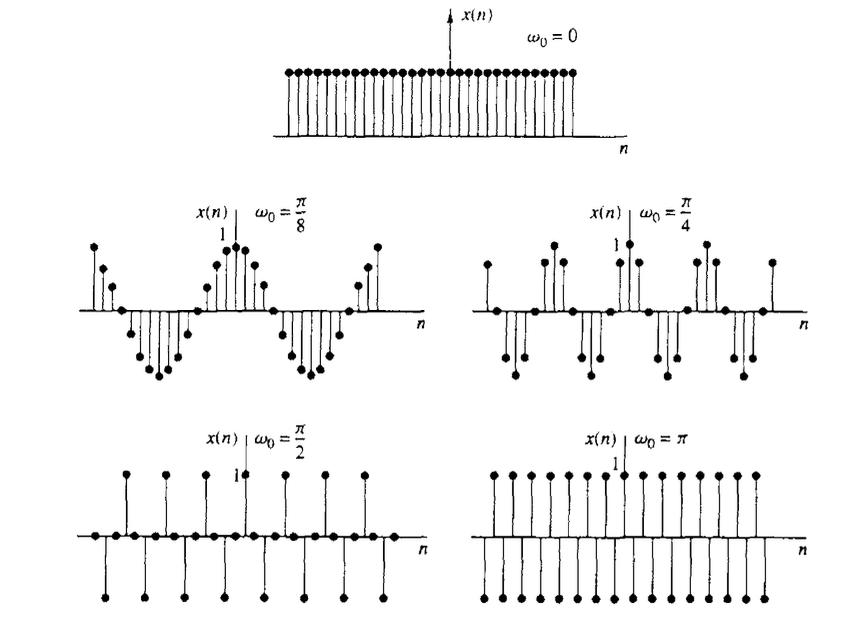
\includegraphics[width=10cm]{dt_freq}
	\caption{Signal showing a DT sine wave with different frequency values.}
	\end{figure}
	
	\section{ADC and DAC}
    Analog to digital conversion is done in the order of sampling, quantizing and encoding.\\
    \textit{Sampling}: This is the conversion of a CT signal into a DT signal by taking samples of the CT wave at distinct time instants.\\
    \textit{Quantization}: Rounding the analog signal to a discrete value. \\
    \textit{Coding}: Converting from the quantized value to a binary value.\\
    
    \subsection{Sampling of Analog Signals}
    In this book the only type of sampling discussed is uniform sampling and is described by:
    \begin{equation}  
	x[n] = x_a(nT), \;\;\;\; -\infty < n < \infty
    \end{equation}
    Periodic sampling establishes a relationship between time (t) and sample (n). The sample period T from the previous equation is related to the sample rate $F_s = 1/T$. 
    \begin{equation}  
	t = nT = \frac{n}{F_s}
    \end{equation}
    As a consequence of equation 15, there exists a relationship between the frequency variable F (or $\Omega$) of analog signals and the frequency variable f or ($\omega$) of DT signals. These following equations show the relationship. When
    \begin{equation}  
	x_a(t) = A \cos(2 \pi Ft + \theta)
    \end{equation}
    is sampled at a rate $F_s = 1/T$ it produces
    \begin{equation}  
	x_a(nT) = x[n] = A \cos(2 \pi FnT + \theta)
    \end{equation}
    \begin{equation}  
	x[n] = A \cos(\frac{2 \pi nF}{F_s} + \theta)
    \end{equation}
    The frequency variables F (CT) and f (DT) are linearly related as:
    \begin{equation}  
	f = \frac{F}{F_s}
    \end{equation}
    or 
    \begin{equation}  
	\omega = \Omega T
    \end{equation}
    DT frequency, f, can be referred to as \textbf{relative or normalized}.
    \begin{figure}[h]
    \centering
	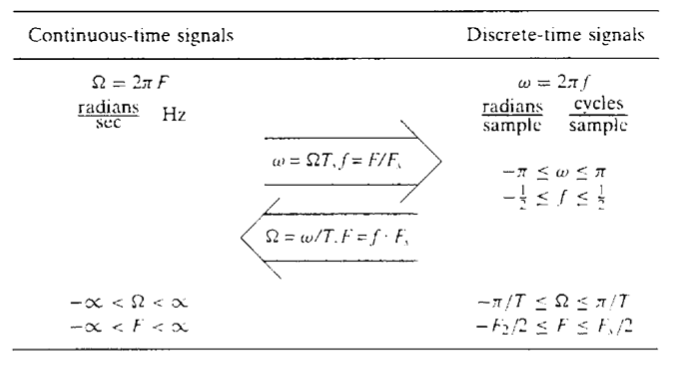
\includegraphics[width=10cm]{freqs}
	\caption{Relations between DT and CT frequencies}
	\end{figure}
	
	\subsection{Sampling Theory}
	The fundamental difference between CT and DT signals is the range of values. Periodic sampling of a CT signal implies a mapping of the infinite frequency range, F (or $\Omega$), to a finite frequency rage, f (or $\omega$), for DT signals. Since the highest frequency in a DT signal is $\omega = \pi$ or $f$ = .5, it follows that, with sampling at $F_s$, the corresponding highest values or F and $\Omega$ are
	\begin{equation}  
	F_{\mathrm{max}} = \frac{F_s}{2} = \frac{1}{2T}
    \end{equation}
    \begin{equation}  
	\Omega_{\mathrm{max}} = \pi F_s = \frac{\pi}{T}
    \end{equation}
    Sampling introduces an ambiguity since the highest frequency in a CT signal that can be uniquely distinguished when sampled at $F_s$ is $F_s/2$. This is the \textbf{nyquist theorem} which states if the sampling rate is not twice the highest frequency in the signal, aliasing will occur.
    \begin{figure}[h]
    \centering
	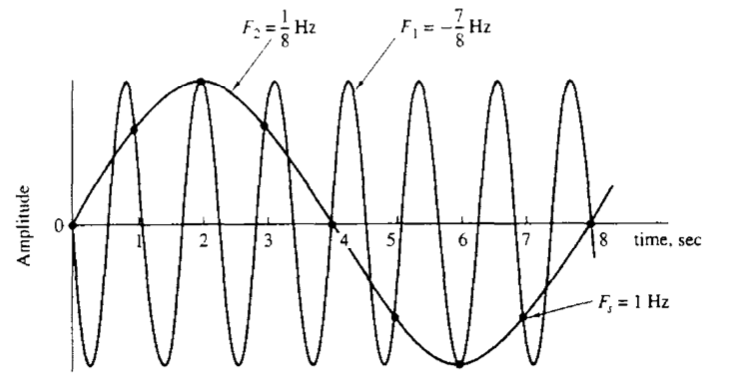
\includegraphics[width=10cm]{alias}
	\caption{Illustration of aliasing}
	\end{figure}
    
    


\end{document} % This is the end of the document